\documentclass{article}
\usepackage[latin1]{inputenc}
\usepackage{amsmath}
\usepackage{amsfonts}
\usepackage{amssymb}
\usepackage{graphicx}
\usepackage{hyperref}
\usepackage{pgfplots}
\begin{document}
	Exercise 1.4.70\\
	Draw pictures that demonstrate that
	$$ \int_{0}^{n}{i^2\mathrm{d}i} \le \sum_{i=0}^{n}{i^2} \le \int_{0}^{n+1}{i^2\mathrm{d}i} $$
	Deduce that
	$$ \sum_{i=0}^{n}{i^2}=\frac{n^3}{3} + O(n^2) $$
	\\
	Proofs:\\
	\\
	\begin{align*}
		\int_{0}^{n}{i^2\mathrm{d}i} &= \frac{i^3}{3}\Big|_0^n = (\frac{n^3}{3}-\frac{0^3}{3}) = \frac{n^3}{3}\\
	\end{align*}	
	\\
	If we take the limit to $\infty$ of the right side over the left side, we will see that the limit goes to 1, which allows us to use the "Squeeze Theorem".\\
	We will need to prove two thigs:\\
	(1) The limit goes to 1.\\
	(2) The summation is greater-equal than the left and less than the right side.\\
	\pagebreak
	\\
	(1)\\
	\\
	\begin{align*}
		\frac{RHS}{LHS} &= \frac{(n+1)^3}{3}*\frac{3}{n^3}\\
		&=\frac{n^{3} + 3n^{2} + 3n + 1}{3}*\frac{3}{n^3}\\
		&=\frac{n^{3} + 3n^{2} + 3n + 1}{1}*\frac{1}{n^3}\\
		&=\frac{n^{3} + 3n^{2} + 3n + 1}{n^3}\\
		\square
	\end{align*}
	\begin{align*}
		\lim_{n->0}{(\frac{n^{3} + 3n^{2} + 3n + 1}{n^3})} = 1\\
	\end{align*}
	\pagebreak
	\\
	(2.1)\\
	\\
	\begin{figure}
		\centering
		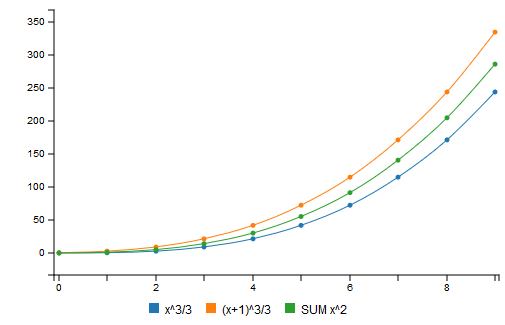
\includegraphics{104070}
		\caption{}
		\label{fig:104070}
	\end{figure}\\
	\url{https://jsfiddle.net/brj8ko2s/1/}\\
	By the picture we see that the summation is always in the middle.
	\\
	\begin{align*}
		\int_{0}^{n}{i^2\mathrm{d}i} \le \sum_{i=0}^{n}{i^2} \le \int_{0}^{n+1}{i^2\mathrm{d}i}\\
		\frac{n^ 3}{3} \le \sum_{i=0}^{n}{i^2} \le \frac{n^{3} + 3n^{2} + 3n + 1}{3}\\
		\frac{n^ 3}{3} \le \sum_{i=0}^{n}{i^2} \le \frac{n^{3}}{3} + \frac{3n^{2} + 3n + 1}{3}\\		
		\frac{n^ 3}{3} \le \sum_{i=0}^{n}{i^2} \le \frac{n^{3}}{3} + O(n^{2})\\
	\end{align*}
	Which means that we can approximate $\sum_{i=0}^{n}{i^2}$ by $\frac{n^ 3}{3}$.
\end{document}